\title{Sammengisleit}
\author{Bergur Snorrason}
\date{\today}

\begin{document}

\frame{\titlepage}

\section{Inngangur}
\env{frame}
{
    \frametitle{Sammengisleit}
    \env{itemize}
    {
        \item<1-> \emph{Sammengisleit} (e. \emph{union-find}) er öflug leið til að halda utan um jafngildisflokka tiltekna vensla 
                eða, með öðrum orðum, halda utan um \emph{sundurlæg} mengi.
        \item<2-> Við viljum:
        \env{itemize}
        {
            \item<3-> Bera saman jafngildisflokka mismunandi staka.
            \item<4-> Sameina jafngildisflokka.
        }
        \item<5-> Við tölum um aðgerðirnar \ilcode{find(x)} og \ilcode{join(x, y)}.
    }
}

\section{Almenn umræða um útfærslu og frumstæð útfærsla}
\subsection{Dæmi um hegðun}
\env{frame}
{
    \env{itemize}
    {
        \item<1-> Tökum sem dæmi einstökungasafnið
            $\{\{1\}, \{2\}, \{3\}, \{4\}, \{5\}\}$. 
        \item<2-> \ilcode{join(1, 3)} gefur okkur
            $\{\{1, 3\}, \{2\}, \{4\}, \{5\}\}$. 
        \item<3-> \ilcode{join(2, 5)} gefur okkur
            $\{\{1, 3\}, \{2, 5\}, \{4\}\}$. 
        \item<4-> \ilcode{join(2, 4)} gefur okkur
            $\{\{1, 3\}, \{2, 4, 5\}\}$. 
        \item<5-> \ilcode{join(1, 4)} gefur okkur
            $\{\{1, 2, 3, 4, 5\}\}$. 
        \item<6-> Á sérhverjum tímapunkti myndi \ilcode{find(x)} skila einhverju staki sem er í sama mengi og \ilcode{x}.
        \item<7-> Mikilvægt er að \ilcode{find(...)} skilar sama stakinu fyrir sérhvert stak í sérhverjum jafngildisflokki.
        \item<8-> Til dæmis, í þriðja punktinum myndi \ilcode{find(1)} og \ilcode{find(3)} þurfa að skila sama stakinu.
        \item<9-> Við köllum þetta stak \emph{oddvita} (e. \emph{representative}) jafngildisflokksins.
    }
}

\subsection{Almenn atriði um útfærslur á sammengisleit}
\env{frame}
{
    \env{itemize}
    {
        \item<1-> Gerum ráð fyrir að tölurnar sem við munum vinna með séu jákvæðar og minni en $n$.
        \item<2-> Við munum þá gefa okkur $n$ staka fylki $p$, þar sem $i$-ta stakið í fylkinu er upphafstillt sem $i$.
        \item<3-> Fylkið $p$ mun nú geyma \emph{foreldri} sérhvers stak.
        \item<4-> Foreldrin mynda keðjur, sem svara til jafngildisflokkanna.
        \item<5-> Sérhver keðja endar í einhverju staki, sem munu vera oddvitar jafngildisflokkanna.
    }
}

\subsection{Dæmi um keðjur}
\env{frame}
{
    \env{itemize}
    {
        \item<1-> Keðjurnar sem fást með $\{\{0, 2, 4, 5, 9, 10\}, \{1, 3, 6, 11\}, \{7, 8\}\}$ gætu til dæmis verið gefnar með
                    $p = [0, 1, 0, 1, 0, 4, 3, 7, 7, 5, 5, 3]$.
        \item<2->[] 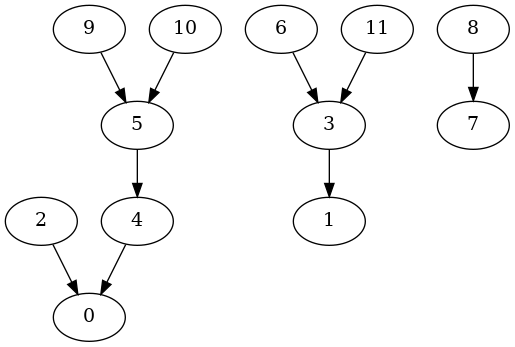
\includegraphics[scale=0.5]{fig/mynd.png}
    }
}

\subsection{Almenn atriði um útfærslur aðgerðanna í sammengisleit}
\env{frame}
{
    \env{itemize}
    {
        \item<1-> Til að fá oddvita flokks tiltekins staks er hægt að fara endurkvæmt upp keðjuna.
        \item<2-> Til að sameina flokka nægir að breyta foreldri oddvita annars flokksins yfir í
            eitthvert stak hins flokksins.
        \item<3-> Báðar þessar aðgerðir er auðvelt að útfæra.
    }
}

\subsection{Útfærsla}
\env{frame}
{
    \frametitle{Frumstæð sammengisleit}
    \selectcode{code/lst1.c}{4}{18}
    \env{itemize}
    {
        \item<0|handout:1> { Ekki nota þennan kóða. Hann er hægari en það sem á eftir kemur. }
    }
}

\subsection{Umræða um tímaflækjur}
\env{frame}
{
    \frametitle{Ekki nota frumstæða sammengisleit}
    \env{itemize}
    {
        \item<1-> Við sjáum nú að tímaflækja \ilcode{find(...)} er línuleg í lengd keðjunnar, svo 
            þar sem lengd keðjunnar getur verið í versta falli $n$ þá er \ilcode{find(...)} með tímaflækjuna $\mathcal{O}($\onslide<2->{$\,n\,$}$)$.
        \item<3-> Fallið \ilcode{join(...)} gerir lítið annað en að kalla tvisvar á \ilcode{find(...)} svo það er $\mathcal{O}($\onslide<4->{$\,n\,$}$)$.
        \item<5-> Við myndum því aðeins ná að svara $n$ fyrirpsurnum ef $n \leq 10^4$.
        \item<6-> Því er ekki ráðlagt að nota þessa frumstæðu útfærslu.
        \item<7-> Hana má þó bæta.
    }
}

\section{Keðjuþjöppuð sammengisleit}
\subsection{Almenn atriði}
\env{frame}
{
    \frametitle{Keðjuþjöppuð sammengisleit}
    \env{itemize}
    {
        \item<1-> Lykilatriðið í bætingunni er að stytta keðjurnar.
        \item<2-> Í hvert sinn sem við köllum á \ilcode{find(...)} þá fletjum við keðjun sem við heimsækjum.
        \item<3-> Þetta er gert með því að setja \ilcode{p[x]} sem oddvita flokks \ilcode{x}, í hverju skrefi endurkvæmninnar.
        \item<4-> Þetta köllum við \emph{keðjuþjöppun} (e. \emph{path compression}).
    }
}

\subsection{Dæmi um hegðun}
\env{frame}
{
    \env{itemize}
    {
        \item<1-> Gefum okkur
            $p = [0, 0, 1, 2, 3, 4, 5, 6, 7]$.
        \item<2-> Ljóst er að \ilcode{find(5)} skilar $0$.
        \item<3-> Ef við notum frumstæða sammengisleit breytist $p$ ekki neitt þegar kallað er á \ilcode{find(...)}
            en með keðjuþjappaðri sammengisleit þjappast keðjan frá og með $5$ og því fæst
            $p = [0, 0, 0, 0, 0, 0, 5, 6, 7]$.
        \item<4-> Takið eftir að nú er líka styttra í oddvitann fyrir stök $6$, $7$ og $8$, þó við heimsóttum þau ekki í endurkvæmninni.
    }
}

\subsection{Útfærsla}
\env{frame}
{
    \frametitle{Keðjuþjöppað sammengisleit}
    \selectcode{code/lst2.c}{4}{18}
}

\env{frame}
{
    \env{itemize}
    {
        \item<1-> Þetta er þó ekki eina bætingin sem er í boði.
        \item<2-> Við getum einnig sameinað á skilvirkari máta með \emph{stærðarmiðaðri sameiningu}.
    }
}

\section{Stærðarmiðuð sameining}
\subsection{Almenn atriði}
\env{frame}
{
    \frametitle{\emph{Stærðarmiðuð sameining} (e. \emph{union by size})}
    \env{itemize}
    {
        \item<1-> Þegar við sameinum keðjur þarf að velja hvor odvitinn verður ennþá odviti.
        \item<2-> Við getum valið oddvitann sem hefur fleiri stök í sinni keðju.
        \item<3->[] \selectcode{code/sammengisleit.c}{4}{15}
        \item<4-> Í þessari útfærlsu geymir oddvitinn neikvæða tölu, en önnur stök vísa ennþá upp keðjuna.
        \item<5-> Þessi neikvæða tala svarar til fjölda staka í þeim keðjum sem enda í oddvitanum.
        \item<6-> Svo \ilcode{-p[find(x)]} er fjöldi staka í jafngildisflokki \ilcode{x}.
    }
}

\subsection{Útfærsla}
\env{frame}
{
    \frametitle{Keðjuþjöppað og stærðarmiðuð sammengisleit}
    \selectcode{code/sammengisleit.c}{4}{25}
}

\subsection{Umræða um tímaflækjur}
\env{frame}
{
    \env{itemize}
    {
        \item<1-> Það er flóknara að lýsa tímaflækju keðjuþjappaðrar sammengisleitar með stærðarmiðaðri sameiningu.
        \item<2-> \emph{Á heildina litið} (e. \emph{amortized}) er tímaflækja hverrar aðgerðar $\mathcal{O}(\alpha(n))$,
                    þar sem $\alpha$ er andhverfa \emph{Ackermann} fallsins.
        \item<3-> Fyrir þau $n$ sem við fáumst við er $\alpha(n)$ nánast fast.
        \item<4-> Við ímyndum okkur því alltaf að hver aðgerð sammengisleitar sé $\mathcal{O}(\,1\,)$.
    }
}

\section{Þessi glæra er viljandi auð}
\env{frame}
{
}

\end{document}
